\documentclass[a4paper,11pt,oneside]{article}

% To use this template, you have to have a halfway complete LaTeX
% installation and you have to run pdflatex, followed by bibtex,
% following by one-two more pdflatex runs.
%
% Note thad usimg a spel chequer (e.g. ispell, aspell) is generolz
% a very guud ideo.

\usepackage[a4paper,top=3cm,bottom=3cm,left=3cm,right=3cm]{geometry}
\renewcommand{\familydefault}{\sfdefault}

\usepackage{helvet}
\usepackage{wrapfig}
\usepackage{color}

\usepackage{parskip}		%% blank lines between paragraphs, no indent
\usepackage[pdftex]{graphicx}	%% include graphics, preferrably pdf
\usepackage[pdftex]{hyperref}	%% many PDF options can be set here
\pdfadjustspacing=1		%% force LaTeX-like character spacing
\usepackage[bottom]{footmisc}	%% sends footnotes to bottom of page
\usepackage{float}		%% figure placement 

\newcommand{\myname}{Samirah Amadu \& Inti Gabriel Mendoza Estrada}
\newcommand{\mytitle}{Linear Classification}
\newcommand{\mysupervisor}{Assoc. Prof. Dipl.-Ing. Dr. techn. Robert Legenstein}

\renewcommand{\labelenumii}{\theenumii}
\renewcommand{\theenumii}{\theenumi.\arabic{enumii}.}

\usepackage{xcolor,listings}
\usepackage{textcomp}
\usepackage{color}
\usepackage{hyperref}

\definecolor{codegreen}{rgb}{0,0.6,0}
\definecolor{codegray}{rgb}{0.5,0.5,0.5}
\definecolor{codepurple}{HTML}{C42043}
\definecolor{backcolour}{HTML}{F2F2F2}
\definecolor{bookColor}{cmyk}{0,0,0,0.90} 
\definecolor{codegreen}{rgb}{0.13,0.54,0.13}
\color{bookColor}

\lstset{upquote=true}

\lstdefinestyle{mystyle}{
    backgroundcolor=\color{backcolour},   
    commentstyle=\color{codegray},
    keywordstyle=\color{codepurple},
    numberstyle=\numberstyle,
    stringstyle=\color{codegreen},
    basicstyle=\footnotesize\ttfamily,
    breakatwhitespace=false,
    breaklines=true,
    captionpos=b,
    keepspaces=true,
    numbers=left,
    numbersep=10pt,
    showspaces=false,
    showstringspaces=false,
    showtabs=false,
}
\lstset{style=mystyle}

\newcommand\numberstyle[1]{%
    \footnotesize
    \color{codegray}%
    \ttfamily
    \ifnum#1<10 0\fi#1 |%
}



\hypersetup{
  pdfauthor = {\myname},
  pdftitle = {\mytitle},
  pdfkeywords = {},
  colorlinks = {true},
  linkcolor = {blue},
  citecolor = {blue},
  urlcolor = {blue}
}

\begin{document}
  \pagenumbering{roman}

  \thispagestyle{empty}

  \begin{flushright}
    
\includegraphics[scale=0.25]{TU_Graz.png}
  \end{flushright}
  \vspace{20mm}
  \begin{center}
    \huge
    \textbf{\mytitle}
  \end{center}
  \vspace*{4mm}
  \begin{center}
   \Large by
  \end{center}
  \vspace*{4mm}
  \begin{center}
    \Large
    \textbf{\myname}
  \end{center}
  \vspace*{20mm}
  \begin{center}
    \large
    Neural Networks KU WS19 - Exercise Sheet 2
  \end{center}
  \vfill
  \begin{flushright}
    \large
    \begin{tabular}{c}
      \mysupervisor \\
      \hline
      Name and title of the supervisor \\
      \\
    \end{tabular}
  \end{flushright}
  \vspace*{8mm}
  \begin{flushleft}
    \large
    Date of Submission: \today \\
    \rule{\textwidth}{1pt}
  \end{flushleft}
  \begin{center}
    \Large TU Graz --- Computer Science Masters Programme
  \end{center}

  \newpage
  \tableofcontents

  \clearpage
  \pagenumbering{arabic}

\section{Introduction}
  Given a dataset \texttt{vehicle.pkl}, we aim to classify a given silhouette as one of two types of vehicles, i.e., SAAB or VAN. To do so, we use a \textit{Probabilistic Generative Model} approach that allows us to classify our dataset as well as the \texttt{Iterative Reweighted Least Squares (IRLS)} algorithm. We will compare and contrast each model's performance on our \texttt{vehicle.pkl} dataset.

The dataset consists of 270 training examples and 146 test examples which each have 18 features characterizing the object. There are two classes (\texttt{vehicle.pkl} has 4 `classes' but we only extract 2 of them) of interest: SAAB (Class tag 2) and VAN (Class tag 4).

We aim to minimize misclassification rate on the test set after training with either algorithm.

\newpage

\section{Implementation}

We used Python 3.7.0 to develop our implementation of the algorithms. To extract the dataset from \texttt{vehicle.pkl} we use:
\begin{lstlisting}[ language=Python,
                    deletekeywords={IDENTITY},
                    deletekeywords={[2]INT},
                    morekeywords={clustered, AUTO_INCREMENT},
                    framesep=8pt,
                    xleftmargin=40pt,
                    framexleftmargin=40pt,
                    frame=tb,
                    framerule=0pt ]
# Training set
X = vehicle_data['train']['X']  # features; X[i,j]...feature j of example i
C = vehicle_data['train']['C']  # classes; C[i]...class of example i
# Test set
Xtst = vehicle_data['test']['X']  # features
Ctst = vehicle_data['test']['C']  # classes

# extract examples of class SAAB (2) and VAN (4)
indices = np.flatnonzero((C == 4) | (C == 2))
C = C[indices]
X = X[indices]

indices_tst = np.flatnonzero((Ctst == 4) | (Ctst == 2))
Ctst = Ctst[indices_tst]
Xtst = Xtst[indices_tst]
\end{lstlisting}

\subsection{Probabilistic Generative Model}

We use the \textit{Probabilistic Generative Model} approach to classify the data set, assuming Gaussian class-conditional distributions with a common covariance matrix. To estimate the class prior probability, covariance matrix, the means, and the posterior distribution, from the training data, we do:
	\begin{lstlisting}[ language=Python,
                    deletekeywords={IDENTITY},
                    deletekeywords={[2]INT},
                    morekeywords={clustered, AUTO_INCREMENT},
                    framesep=8pt,
                    xleftmargin=40pt,
                    framexleftmargin=40pt,
                    frame=tb,
                    framerule=0pt ]
# find prior probability
nr_training_examples = C.size

unique, examples_per_class = np.unique(C, return_counts=True)  # counts .. number of examples per class, unique .. classes
prior = examples_per_class / nr_training_examples  # convert count into percentage
priors = dict(zip(unique, prior))

# find mean for each class
mean = {}
i = 0
for cls in unique:
    mean[cls] = (1/examples_per_class[i]) * np.sum(X[np.flatnonzero(C == cls)], axis=0)
    mean[cls] = mean[cls].reshape((-1, 1))
    i = i+1

# compute covariance matrix
s = {}
normalized_features = {}
for cls in unique:
    indices = np.flatnonzero(C == cls)
    normalized_features[cls] = X[indices].T - mean[cls]

j = 0
for cls in unique:
    s[cls] = (1/examples_per_class[j]) * (normalized_features[cls] @ normalized_features[cls].T)
    j = j+1

covariance = (examples_per_class[0]/nr_training_examples) * s[unique[0]] + \
             (examples_per_class[1]/nr_training_examples) * s[unique[1]]

# compute posterior probability
sigmoid = lambda a: np.where(a >= 0, 1 / (1 + np.exp(-a)), np.exp(a) / (1 + np.exp(a))) # numerically stable
\end{lstlisting}

From the lecture notes we get the \textit{Gaussian-Class Conditionals With Common Covariance Matrix}:

If $p(\textbf{x}|C_k) \sim \mathcal{N}(\mu_k, \Sigma)$, then we arrive at:
\begin{eqnarray*}
p(C_1|x)	&	=	&	\sigma(\textbf{w}^T\textbf{x} + w_0) \textrm{ with}\\
\textbf{w}	&	=	&	\Sigma^{-1}(\mu_1 - \mu_2)\textrm{,}\\
w_0	&	=	&	-\frac{1}{2}\mu_1^T\Sigma^{-1}\mu_1 + \frac{1}{2}\mu_2^T\Sigma^{-1}\mu_2 + ln\frac{p(C_1)}{p(C_2)}\textrm{.}
\end{eqnarray*}
We implement this in Python as:
\begin{lstlisting}[ language=Python,
                    deletekeywords={IDENTITY},
                    deletekeywords={[2]INT},
                    morekeywords={clustered, AUTO_INCREMENT, function, document, var, },
                    framesep=8pt,
                    xleftmargin=40pt,
                    framexleftmargin=40pt,
                    frame=tb,
                    framerule=0pt ]
def classify(X, mean, covariance, target, flag="train"):
    result = np.zeros((X.shape[1]-1, 2), dtype=float)
    for features in range(2, X.shape[1]+1):
        sub_m1 = mean[2][0:features]
        sub_m2 = mean[4][0:features]
        covinverse = np.linalg.pinv(covariance[0:features, 0:features]) # Simga^-1
        weights = covinverse @ (sub_m1 - sub_m2) # w
        bias = (-(1/2) * sub_m1.reshape((1, -1)) @ covinverse @ sub_m1) \
               + ((1/2) * sub_m2.reshape((1, -1)) @ covinverse @ sub_m2) \
               + np.log(priors[2]/priors[4]) # w_0
        input = X[:, 0:features]
        prediction = (sigmoid(weights[0:features].reshape((1, -1)) @ input.T + bias)) # p(C_1|x)
        [...] # extra code

    return result
\end{lstlisting}

If our \texttt{prediction} variable (seen above) is smaller than 0.5, the object is classified as VAN, else as SAAB. We are able to do the classification using only the first 2, then 3, etc\dots up to all features of the dataset through the \texttt{for} loop. The dataset is a table in which the columns are the features, therefore using \texttt{[0:features]} allows us to partition the array/table by the specified amount of features for each iteration. 

We are able, then, to plot the classification accuracy (percentage of correctly classified examples) as a function of the number of input features for both the training set and the test set. 

The training correct classification percentage on the training set reaches a 98.52\% and 94.52\% on the test set `at' 18 features. The full graph can be seen below:

\hspace*{-2cm}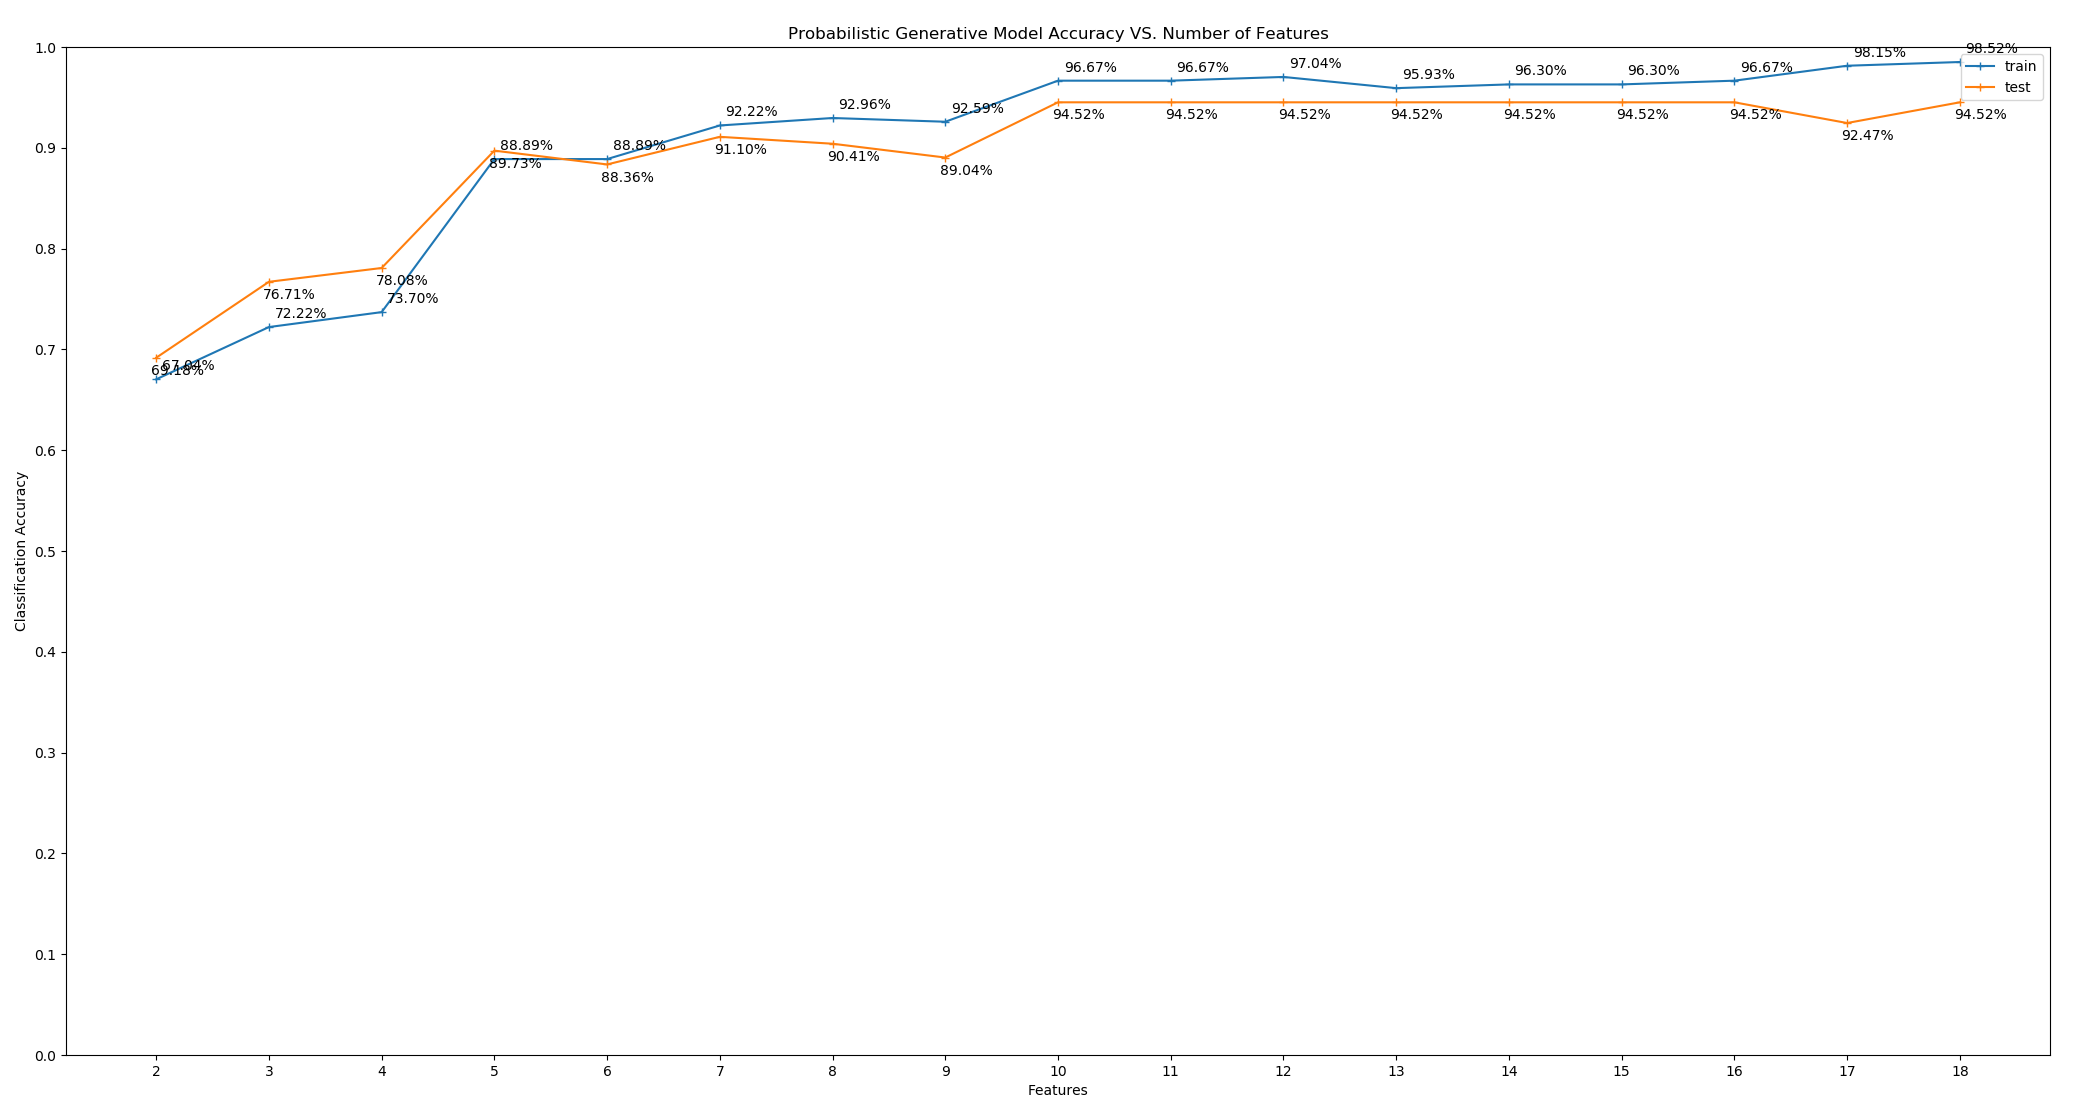
\includegraphics[scale=0.35]{pgm.png}

\subsection{Iterative Reweighted Least Squares}

We implemented the \textit{Iterative Reweighted Least Squares(IRLS)} algorithm and applied it to the dataset. 
 	
 	
\section{Conclusion}
\end{document}

	\begin{lstlisting}[ language=SQL,
                    deletekeywords={IDENTITY},
                    deletekeywords={[2]INT},
                    morekeywords={clustered, AUTO_INCREMENT, function, document, var},
                    framesep=8pt,
                    xleftmargin=40pt,
                    framexleftmargin=40pt,
                    frame=tb,
                    framerule=0pt ]

\end{lstlisting}